%===============================================================
% Template using official colors of Czech Technical University.
% They are defined by new graphical manual - 2017.
% Specially designed for Laboratory of Structure of Biomolecules
% Share and modify as you like. Keep the name of the author.
% It is forbidden to use the template commercially.
% Author: Martin Malý.
% Published: 23.9.2017.
%===============================================================

\documentclass{beamer}
\usepackage[utf8]{inputenc}
\usepackage{tikz}
\usetikzlibrary{calc}
\usepackage{appendixnumberbeamer}

\usetheme{Madrid}

\definecolor{cvut_navy}{HTML}{0065BD}
\definecolor{cvut_blue}{HTML}{6AADE4}
\definecolor{cvut_gray}{HTML}{156570}

\setbeamercolor{section in toc}{fg=black,bg=white}
\setbeamercolor{alerted text}{fg=cvut_blue}
\setbeamercolor*{palette primary}{bg=cvut_navy,fg=gray!20!white}
\setbeamercolor*{palette secondary}{bg=cvut_blue,fg=white}
\setbeamercolor*{palette tertiary}{parent=palette primary}
\setbeamercolor*{palette quaternary}{fg=green,bg=gray!5!white}

\setbeamercolor*{sidebar}{fg=cvut_navy,bg=gray!15!white}


\setbeamercolor{titlelike}{parent=palette primary}
\setbeamercolor{frametitle}{parent=palette primary}

\setbeamercolor*{separation line}{}
\setbeamercolor*{fine separation line}{}

\setbeamertemplate{navigation symbols}{}


\usepackage{eqnarray,amsmath}
\usepackage{amsfonts}
\usepackage{amssymb}
\usepackage{graphicx}
\usepackage{lmodern} % pro pismo tucne a zaroven kurziva
\usepackage{bm} % pro pismo tucne a zaroven kurziva
\usepackage{epstopdf}
\usepackage{changepage}
\usepackage{array,booktabs}

%====================================================
%========== DEFINITION OF AUTHORS ETC...=============
%====================================================
\author[František Boháček]{František Boháček}
\title[NSV semestral project]{SSD1306 display control over I²C}
\date[2. 2. 2024]{2. 2. 2024}

%====================================================
%========== BEGINNING OF DOCUMENT ===================
%====================================================
\begin{document}

\begin{frame}
    \titlepage
    \begin{center}
          \includegraphics[height=1.5cm]{files/symbol_cvut_plna_samostatna_verze.pdf}
    \end{center}
\end{frame}
\logo{\includegraphics[height=1cm]{files/symbol_cvut_plna_samostatna_verze.pdf}}

\begin{frame}
    \frametitle{I²C entities}

    \begin{itemize}
      \item Entities for general use
      \item Support for arbitration clock stretching
      \item Error reporting
    \end{itemize}

    \begin{center}
      \includegraphics[width=0.4\textwidth]{blocks/svg/master.pdf}
      \includegraphics[width=0.4\textwidth]{blocks/svg/slave.pdf}
    \end{center}
\end{frame}

\begin{frame}
  \frametitle{I²C slave - block}

  \begin{center}
    \hspace{1.8cm}
    \includegraphics[width=0.65\textwidth]{blocks/svg/slave.pdf}
  \end{center}
\end{frame}

\begin{frame}
  \frametitle{I²C slave - structure}

  \begin{center}
    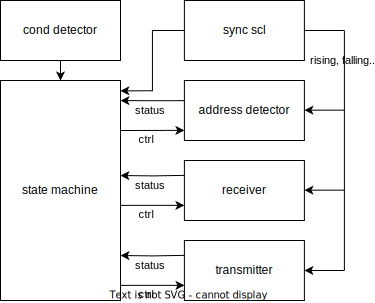
\includegraphics[width=0.65\textwidth]{img/i2c_slave.pdf}
  \end{center}
\end{frame}

\begin{frame}
  \frametitle{I²C master - block}

  \begin{center}
    \hspace{1.5cm}
    \includegraphics[width=0.65\textwidth]{blocks/svg/master.pdf}
  \end{center}
\end{frame}

\begin{frame}
  \frametitle{I²C master - structure}

  \begin{center}
    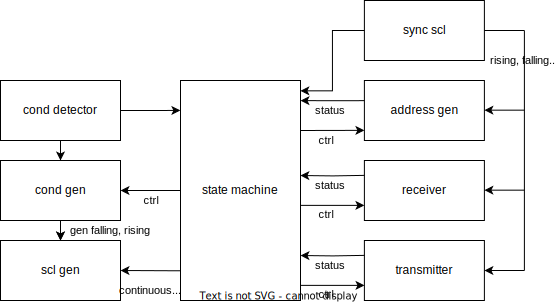
\includegraphics[width=0.9\textwidth]{img/i2c_master.pdf}
  \end{center}
\end{frame}

\begin{frame}
  \frametitle{Testing - simulation}
  \begin{columns}
    \begin{column}{0.4\textwidth}
        \begin{itemize}
            \item VUnit
            \item Automated testing
        \end{itemize}
    \end{column}
    \begin{column}{0.6\textwidth}
      \includegraphics[width=0.8\textwidth]{img/vunit_run.png}
    \end{column}
  \end{columns}
\end{frame}

\begin{frame}
  \frametitle{Testing - slave with microcontroller - registers}

  \begin{columns}
    \begin{column}{0.5\textwidth}
      \begin{itemize}
        \item Microcontroller as master
        \item 20 registers
        \item Read, write
        \item First write address
        \item Consecutive read/write
      \end{itemize}
    \end{column}

    \begin{column}{0.5\textwidth}
      \includegraphics[width=0.7\textwidth]{img/tiva-c-kit.png}
    \end{column}
  \end{columns}
\end{frame}

\begin{frame}
  \frametitle{Testing - master with SSD1306 display - diagram}

  \begin{center}
    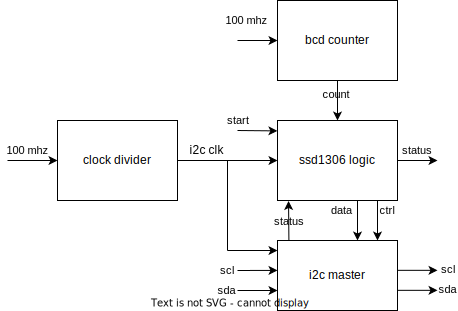
\includegraphics[width=0.7\textwidth]{img/ssd1306_master.pdf}
  \end{center}
\end{frame}

\begin{frame}
  \frametitle{Testing - master with SSD1306 display - photo}

  \begin{center}
    \includegraphics[width=0.85\textwidth]{img/fpga-board-ssd1306.jpg}
  \end{center}
\end{frame}

\begin{frame}[plain]
    \frametitle{Thank you for your attention}
    Thank you for your attention.
\end{frame}

\appendix


\end{document}
% =============================================================
% =========================== END =============================
% =============================================================
